\documentclass[10pt]{article}
\usepackage[margin=0.6in]{geometry}
\usepackage{graphicx}
\usepackage{booktabs}
\usepackage{parskip}
\usepackage{hyperref}
\usepackage{enumitem}
\setlength{\parindent}{0pt}
\setlist{nosep,leftmargin=1.2em}
\setlength{\parskip}{4pt}

\begin{document}
\csname @@input\endcsname trial_stats.tex
\begin{center}
{\Large\textbf{ECE 5755 Lab 2: Tiling/Blocking, Quantization and Attention}}\\[1pt]
\small Intel Xeon Silver 4514Y (Sapphire Rapids), gcc 13.3, Top-down level 1--2 via \texttt{toplev.py}
\end{center}
\textbf{Name:} Abiola \hfill \textbf{NetID:} ab3394

\section*{1. Implementation summary}
\textbf{\texttt{matmul\_blocking}} splits $C=AB$ into $B_I\times B_K$ tiles of A, $B_K\times B_J$ tiles of B and $B_I\times B_J$ tiles of C (outer loops $i_0,k_0,j_0$). Inside a tile the loops run in $i$-$k$-$j$ order: \texttt{A[i][k]} is held in a register while \texttt{B[k][j..]} and \texttt{C[i][j..]} are streamed with unit stride, so every fetched cache line is fully used. The final tile is $64\times256\times32$: the B tile is $32\times256\times4$\,B $=32$\,KB and fits in the 48\,KB L1d, and it is reused by all 64 rows of the A tile before being evicted. Edge tiles are clipped, so any shape works (tested on $131\times77 \cdot 77\times301$ against \texttt{matmul}).
\textbf{\texttt{matmul\_quant}} unpacks four 8-bit values per \texttt{unsigned int}, most significant byte first, with a shift and \texttt{\&0xFF} mask (\texttt{0x01020304}$\,\to[1,2,3,4]$ multiplies rows $4w..4w{+}3$ of B), accumulates in a 64-bit integer and casts to float.
\textbf{\texttt{scaled\_dot\_product\_attention}} computes $\mathrm{softmax}(QK^T/\sqrt{d})V$ row by row, subtracting the row maximum before \texttt{expf} for numerical stability. All 19 Unity tests pass, including new tests for edge tiles, the handout's quantization example, uniform attention, and empty inputs to \texttt{flatten} and \texttt{linear} (which now return \texttt{NULL}).

\section*{2. Profiling process}
\begin{itemize}
\item \textbf{Program under test.} \texttt{perf/matmul\_naive.c}, \texttt{perf/matmul\_blocking.c} and \texttt{perf/matmul\_blocking\_ijk.c} each build two random $N\times N$ float matrices, then call one kernel \texttt{reps} times in a loop ($N$=256: 100, 1024: 3, 2048: 1), freeing each result, so the matmul dominates runtime. Setup alone (allocation, \texttt{rand()}, program start; measured with reps $=0$) takes 0.1--0.3\,s, i.e.\ $\le$6\% of every run except the fastest 256$^2$ \texttt{-O2} runs ($\sim$10\%). Tile sizes are compile-time macros (\texttt{-DBLOCK\_SIZE\_I=...}), so one source file builds every tiled variant.
\item \textbf{How it is measured.} The program is pinned to one core with \texttt{taskset -c 0}, and toplev collects Top-down counters for that core only:\\
\texttt{toplev.py --core S0-C0 -l2 -v --no-desc --force-cpu spr taskset -c 0 ./prog N reps}\\
Runtime comes from separate runs under \texttt{/usr/bin/time} (wall-clock \emph{real} time), one job at a time. \textbf{Every toplev and timing measurement is repeated in \toplevTrials{} independent trials} (separate program runs); the figure and table report the mean, and the table also gives the standard deviation. Every program is built at the Makefile default (\texttt{-O0}, as in Lab 1) and again at \texttt{-O2}, because \texttt{-O0} hides cache effects (Section 4). Everything is scripted in \texttt{scripts/run\_perf.sh}; raw outputs are in \texttt{perf\_results/}.
\item \textbf{Inputs.} $N$=256 (3 matrices = 768\,KB, larger than L1 but within L2), 1024 (12\,MB, larger than L2) and 2048 (48\,MB, larger than L3).
\item \textbf{Implementations.} Lab 1 \texttt{matmul} ($ijk$); a tiled version with $ijk$ order inside the tile (my first attempt); tiled $ikj$ with small $16\times64\times16$ tiles; tiled $ikj$ with $64\times256\times32$ tiles (final). A sweep of 27 tile shapes (\texttt{scripts/sweep\_tiles.sh}) chose the final tile.
\end{itemize}

\section*{3. Results}
\textbf{Reading the labels.} Each row in Figure 1 and Table 2 is ``$N^2$ \textit{flag} \textit{implementation}'': $N$ is the matrix size and \textit{flag} the gcc optimization level. Implementations are named by the order of their three nested loops, outermost first: $i$ is a row of A and C, $j$ a column of B and C, and $k$ the dimension summed over (a column of A and a row of B). All of them compute \texttt{C[i][j] += A[i][k] * B[k][j]}; only the loop order and tiling differ.
\begin{center}
\small
\begin{tabular}{@{}llll@{}}
\toprule
Label & Loops (outer $\to$ inner) & Tile $B_I\times B_J\times B_K$ & Innermost loop walks \\
\midrule
matmul (Lab 1, ijk) & $i,j,k$ (no tiling) & -- & down a column of B (new row every step) \\
tiled ijk 64x256x32 & tiles $i_0,j_0,k_0$; in tile $i,j,k$ & $64\times256\times32$ & down a column of B, within the tile \\
tiled ikj 16x64x16 & tiles $i_0,k_0,j_0$; in tile $i,k,j$ & $16\times64\times16$ & along a row of B and C (unit stride) \\
tiled ikj 64x256x32 (final) & tiles $i_0,k_0,j_0$; in tile $i,k,j$ & $64\times256\times32$ & along a row of B and C (unit stride) \\
\bottomrule
\end{tabular}\\[2pt]
\textbf{Table 1.} Implementations compared. The final row is the submitted \texttt{matmul\_blocking}.
\end{center}
\begin{center}
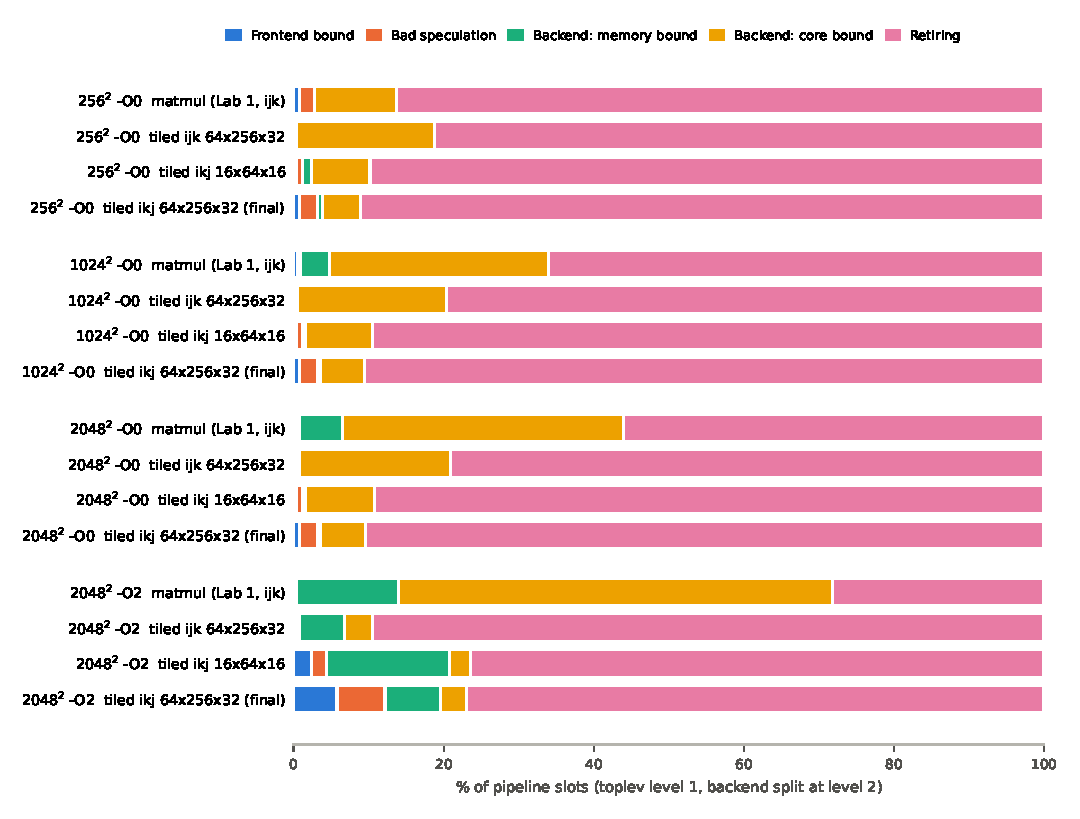
\includegraphics[width=0.84\linewidth]{topdown.pdf}\\[-2pt]
\small\textbf{Figure 1.} Top-down breakdown per implementation and input (\% of pipeline slots; backend split into memory/core at level 2), mean of \toplevTrials{} trials. Per-segment standard deviation across trials: median \toplevMedSd{}, max \toplevMaxSd{} percentage points.
\end{center}

\begin{center}
\small
\begin{tabular}{@{}rlrrrrrr@{}}
\toprule
 & & \multicolumn{3}{c}{\texttt{-O0} (Makefile default)} & \multicolumn{3}{c}{\texttt{-O2}} \\
$N$ & Implementation & real s & s/call & speedup & real s & s/call & speedup \\
\midrule
\csname @@input\endcsname runtime_table.tex
\bottomrule
\end{tabular}\\[2pt]
\textbf{Table 2.} Wall-clock time of the whole program, mean $\pm$ standard deviation over \toplevTrials{} trials (reps $=$ 100 / 3 / 1 for $N$ = 256 / 1024 / 2048); speedup relative to Lab 1 \texttt{matmul}.
\end{center}

\section*{4. Discussion}
\textbf{\texttt{matmul\_blocking} vs.\ \texttt{matmul}.} The final blocked kernel is 2.2$\times$, 2.8$\times$ and 3.4$\times$ faster than \texttt{matmul} at $N$=256, 1024 and 2048 (\texttt{-O0}), and 1.7$\times$, 2.6$\times$ and 3.1$\times$ faster at \texttt{-O2}. The gain grows with $N$: per call, \texttt{matmul} slows down 9.4$\times$ from 1024 to 2048 at \texttt{-O0} (9.7$\times$ at \texttt{-O2}) for 8$\times$ the work, while the blocked kernel scales by 8.0--8.1$\times$. Its runtime therefore stays proportional to the FLOP count even after the working set no longer fits in L2 (1024) or L3 (2048).

\textbf{Why \texttt{matmul} is slow (Core/Memory bound).} In \texttt{matmul} the inner $k$ loop reads \texttt{B[k][j]} down a column. Each B row is a separate allocation, so every iteration touches a new cache line (and a new 4\,KB page every iteration for $N\geq1024$) and uses only 4 of its 64 bytes. That is poor spatial locality, and it shows up as Memory\_Bound rising with $N$ (0\%$\to$3.8\%$\to$5.6\% at \texttt{-O0}; 6.3\%$\to$13.6\% from 1024 to 2048 at \texttt{-O2}). The larger cost is Core\_Bound (29--38\% at \texttt{-O0} for $N\geq1024$, 58\% at \texttt{-O2}). Every iteration adds into the same accumulator (\texttt{C[i][j]} kept in memory at \texttt{-O0}, \texttt{sum} in a register at \texttt{-O2}), forming a loop-carried dependence chain of FP adds over all $N$ values of $k$. The out-of-order core cannot overlap iterations, so execution ports sit idle while each add waits for the previous one, and the column loads that miss in L1 lengthen each step of the chain.

\textbf{Why tiling + $ikj$ helps.} In the $ikj$ tile loop, consecutive iterations write different \texttt{C[i][j]} elements, so they are independent and the core issues them back-to-back. Core\_Bound drops to 5--6\% and Retiring rises to 90--91\% at \texttt{-O0}, for every $N$. B and C are accessed with unit stride (each line fully used, hardware prefetcher friendly), and the 32\,KB B tile is reused by 64 rows of A from L1 before eviction. Memory\_Bound therefore stays under 1\% at \texttt{-O0}, and at \texttt{-O2} is 7.4\% at $N$=2048 versus 13.6\% for \texttt{matmul}, even though the matrices are larger than L3.

\textbf{Comparing implementations.} \emph{At \texttt{-O0}, loop order matters more than tiling.} The tiled-$ijk$ variant has the same tiles but keeps the column walk and the dependent accumulation chain: it is still 20\% Core\_Bound and only 1.4--2.1$\times$ faster than \texttt{matmul}. At \texttt{-O2} the gap narrows. gcc keeps tiled-$ijk$'s partial sum in a register and its chain is only $B_K$=32 adds long, so it is 89--90\% Retiring and 2.2--2.6$\times$ faster than \texttt{matmul}. It is nevertheless 17--20\% slower than the final kernel (5.22 vs.\ 4.36\,s at $N$=2048): \texttt{objdump} shows 9 instructions per multiply-add (it reloads the row pointer \texttt{B[k]} and has two loop-exit branches) versus 7 for $ikj$. High Retiring means the slots do useful work, not that little work is needed. \emph{Tile size matters little here.} At \texttt{-O0} the small $16\times64\times16$ and large $64\times256\times32$ tiles are within 3\% of each other, and a 27-point tile sweep at $N$=1024 spanned only 1.83--1.97\,s, because unoptimized code spends 24 instructions per multiply-add (from \texttt{objdump}) on stack traffic. At \texttt{-O2} the small tile is 3\% slower for $N\geq1024$ and is 16.5\% Memory\_Bound versus 7.4\%: each B tile is reused by only 16 rows of A, so B is streamed from L2/L3 four times as often. At $N$=256, where everything fits in L2, the small tile is marginally faster (0.78 vs.\ 0.80\,s).

\textbf{Remaining bottleneck.} At \texttt{-O2} the final kernel is 77\% Retiring, with the rest split between Memory\_Bound (7\%), Bad\_Speculation (6\%), Frontend\_Bound (6\%) and Core\_Bound (3\%). Its scalar inner loop does one multiply-add per 7 instructions, and \texttt{-fopt-info-vec} confirms gcc does not vectorize it at \texttt{-O2}; SIMD (AVX-512, 16 floats per instruction) would be the next step.

\textbf{Effect of input size.} At $N$=256 all three matrices fit in L2, so \texttt{matmul} is already 86\% Retiring at \texttt{-O0} and blocking gains less (2.2$\times$ at \texttt{-O0}, 1.7$\times$ at \texttt{-O2}). Larger inputs make the baseline's poor locality costlier, while the blocked kernel's profile stays flat.

\section*{5. Issues and debugging}
\begin{itemize}
\item \textbf{Quantization byte order.} My first \texttt{matmul\_quant} extracted the least significant byte as element 0. The provided test uses symmetric words (\texttt{0x01010101}), so it passed anyway. A new test built from the handout's \texttt{0x01020304} example returned 12340 instead of 43210, which exposed the reversed order. I fixed the shift to $(3-e)\cdot 8$.
\item \textbf{Ineffective first blocking attempt.} My first tiled kernel ($ijk$ inside tiles) was only 1.4$\times$ faster at \texttt{-O0}; its 20\% Core\_Bound pointed to the accumulation chain and led to the $ikj$ rewrite.
\item \textbf{toplev measured nothing on the login node} (\texttt{perf\_event\_paranoid}=4). Moving to the Slurm node fixed it. The Makefile's toplev command originally profiled \texttt{S0-C0} without pinning the program, so I added \texttt{taskset -c 0}. Jobs are limited to 5 minutes and all pin to CPU 0, so data collection was split into sequential \texttt{srun} jobs.
\item \textbf{Code alignment skewed my first \texttt{-O2} data.} My first \texttt{-O2} profiles showed the tiled kernels 25--43\% Frontend\_Bound. Repeated trials agreed with each other but not with the first: Frontend\_Bound fell below 6\% and the tiled kernels ran 16--36\% faster. \texttt{objdump} showed identical instructions; a small edit to \texttt{main()} had moved \texttt{matmul\_blocking} 32 bytes, so the hot loop that had straddled a 64-byte boundary (0x2938--0x2954) now sits inside one (0x2958--0x2974). The frontend fetches decoded uops in 64-byte windows, so the old layout most likely needed two fetches per iteration. All \texttt{-O2} results here are 3 trials of the current binaries (old data in \texttt{perf\_results/old\_layout\_O2/}).
\item \textbf{Noise.} Repeating the tile sweep three times showed $\sim$5\% run-to-run variation, larger than most differences between tile shapes. I therefore chose the final tile on cache-capacity reasoning among the statistically tied fastest shapes.
\item \textbf{Attention.} The score buffer was a variable-length array on the stack. I replaced it with \texttt{malloc} so long sequences cannot overflow the stack.
\end{itemize}

\section*{6. AI usage statement}
The code implementation for this lab (\texttt{matmul\_blocking}, \texttt{matmul\_quant}, \texttt{scaled\_dot\_product\_attention} and the accompanying tests) was developed with the assistance of an AI coding assistant (Claude Code, Anthropic). All code was compiled, tested and profiled on the course machines, and the results reported here are from those runs.
\end{document}
